\documentclass{article}
\usepackage{tikz} 
\usepackage[utf8]{inputenc}
\usepackage{amsmath}
\usepackage{listings}
\usepackage{amsfonts}
\usepackage{amssymb}
\usepackage{tabularx}
\usepackage{enumitem}
\usepackage{algorithm}% http://ctan.org/pkg/algorithm
\usepackage[noend]{algpseudocode}% http://ctan.org/pkg/algorithmicx
\usepackage[margin=0.7in]{geometry}
\usepackage{tikz}

\usepackage{graphicx}
\usetikzlibrary{arrows,positioning} 
\usepackage{subcaption}
\thispagestyle{empty}
\usepackage{multicol,caption}
\pgfarrowsdeclarecombine{ring}{ring}{}{}{o}{o}

\DeclareMathOperator{\ringarrow}{\raisebox{0.5ex}{\tikz[baseline]{\draw[ring->](0,0)--(2em,0);}}}

\tikzset{
    %Define standard arrow tip
    >=stealth',
    %Define style for boxes
    observed/.style={
           circle,
           rounded corners,
           draw=black, thick,
           minimum width=2.2em,
           minimum height=2.2em,
           font=\footnotesize,
           text centered,
           fill=blue!20!white},
     latent/.style={
           circle,
           rounded corners,
           draw=black, thick, dashed,
           minimum width=2.2em,
           minimum height=2.2em,
           font=\footnotesize,
           text centered,
           fill=black!10!white
           },
    % Define arrow style
    pil/.style={
           o->,
           thick,
           shorten <=2pt,
           shorten >=2pt,},
    sh/.style={ shade, shading=axis, left color=red, right color=green,
    shading angle=45 }
    
}
   
\begin{document}
\def\ci{\perp\!\!\!\perp} % from Wikipedia


\begin{figure}
\centering
\begin{subfigure}[t]{0.24\textwidth}
\centering
\caption{Counfounded}
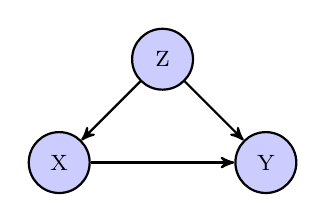
\begin{tikzpicture}[->,shorten >=0pt,shorten <=0pt,node distance=3em,thick,main node/.style={observed}, lt/.style={latent}]
\node[main node](1){Z};
\node[main node, below left=of 1](2){X};
\node[main node, below right=of 1](3){Y};
\path[]
	(1) edge (2)
	(1) edge (3)
	(2) edge (3);
\end{tikzpicture}
\end{subfigure}
\begin{subfigure}[t]{0.24\textwidth}
\centering
\caption{M-graph}
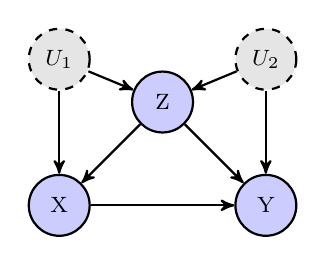
\begin{tikzpicture}[->,shorten >=0pt,shorten <=0pt,node distance=3em,thick,main node/.style={observed}, lt/.style={latent}]
\node[main node](1){Z};
\node[main node, below left=of 1](2){X};
\node[main node, below right=of 1](3){Y};
\node[lt, above=of 2](4){$U_1$};
\node[lt, above=of 3](5){$U_2$};
\path[]
	(1) edge (2)
	(1) edge (3)
	(2) edge (3)
	(4) edge (2) edge (1)
	(5) edge (3) edge (1);
\end{tikzpicture}
\end{subfigure}
\begin{subfigure}[t]{0.24\textwidth}
\centering
\caption{Front door criterion}
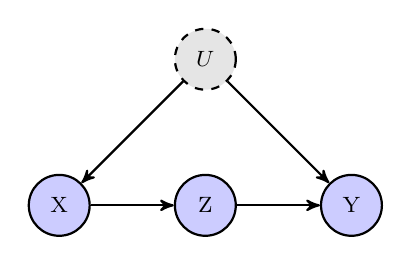
\begin{tikzpicture}[->,shorten >=0pt,shorten <=0pt,node distance=3em,thick,main node/.style={observed}, lt/.style={latent}]
\node[lt](1){$U$};
\node[main node, below=of 1](4){Z};
\node[main node, left=of 4](2){X};
\node[main node, right=of 4](3){Y};
\path[]
	(1) edge (2) edge (3)
	(2) edge (4)
	(4) edge (3);
\end{tikzpicture}
\end{subfigure}
\begin{subfigure}[t]{0.24\textwidth}
\centering
\caption{Instrumental}
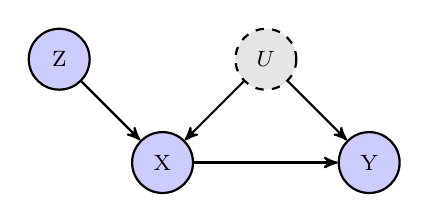
\begin{tikzpicture}[->,shorten >=0pt,shorten <=0pt,node distance=3em,thick,main node/.style={observed}, lt/.style={latent}]
\node[main node](1){Z};
\node[main node, below right=of 1](2){X};
\node[lt, above right=of 2](4){$U$};
\node[main node,  below right=of 4](3){Y};
\path[]
	(1) edge (2)
	(2) edge (3)
	(4) edge (2) edge (3);
\end{tikzpicture}
\end{subfigure}
\end{figure}

\end{document}
\begin{subfigure}[b]{0.24\textwidth}
\centering
\caption{Post-interventional}
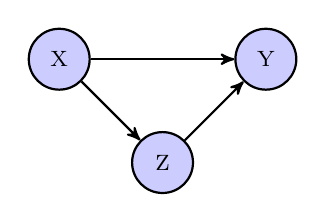
\begin{tikzpicture}[->,shorten >=0pt,shorten <=0pt,node distance=3em,thick,main node/.style={observed}, lt/.style={latent}]

\node[main node](2){X};
\node[main node, below right=of 2](1){Z};
\node[main node, above right=of 1](3){Y};

\path[]
	(2) edge (1)
	(1) edge (3)
	(2) edge (3);
\end{tikzpicture}
\end{subfigure}